\chapter{Pengujian}
Program yang dibuat dapat menyelesaikan papan Queens LinkedIn dengan masukan berupa file \texttt{.txt} melalui antarmuka GUI berbasis SFML. Berikut adalah hasil pengujian menggunakan 5 test case yang berbeda, beserta penanganan input tidak valid.

\section{Test 1: Papan berukuran $9\times 9$ (in1.txt)}
\begin{table}[H]
    \centering
    \begin{minipage}{0.45\textwidth}
        \centering
        \captionof{table}{Input Test 1}
        \renewcommand{\arraystretch}{1.2}
        \setlength{\tabcolsep}{40pt}
        \begin{tabular}{|l|}
            \hline
            \phantom{text}\\
            AAABBCCCD\\
            ABBBBCECD\\
            ABBBDCECD\\
            AAABDCCCD\\
            BBBBDDDDD\\
            FGGGDDHDD\\
            FGIGDDHDD\\
            FGIGDDHDD\\
            FGGGDDHHH\\
            \phantom{text}\\
            \hline
        \end{tabular}
    \end{minipage}
\end{table}

Program menyediakan dua format output: file teks (.txt) dan gambar (.png). Output teks berisi papan dengan posisi queen ditandai \texttt{\#}, waktu pencarian, dan jumlah iterasi. Output gambar menampilkan visualisasi GUI.

\subsection*{Output sebagai File TXT}
\begin{lstlisting}[basicstyle=\ttfamily\small]
AAABBCC#D
ABBB#CECD
ABBBDC#CD
A#ABDCCCD
BBBBD#DDD
FGG#DDHDD
#GIGDDHDD
FG#GDDHDD
FGGGDDHH#

Waktu pencarian: 1461 ms
Banyak kasus yang ditinjau: 323741637 kasus
\end{lstlisting}

\subsection*{Output sebagai Gambar (PNG)}
\begin{figure}[H]
    \centering
    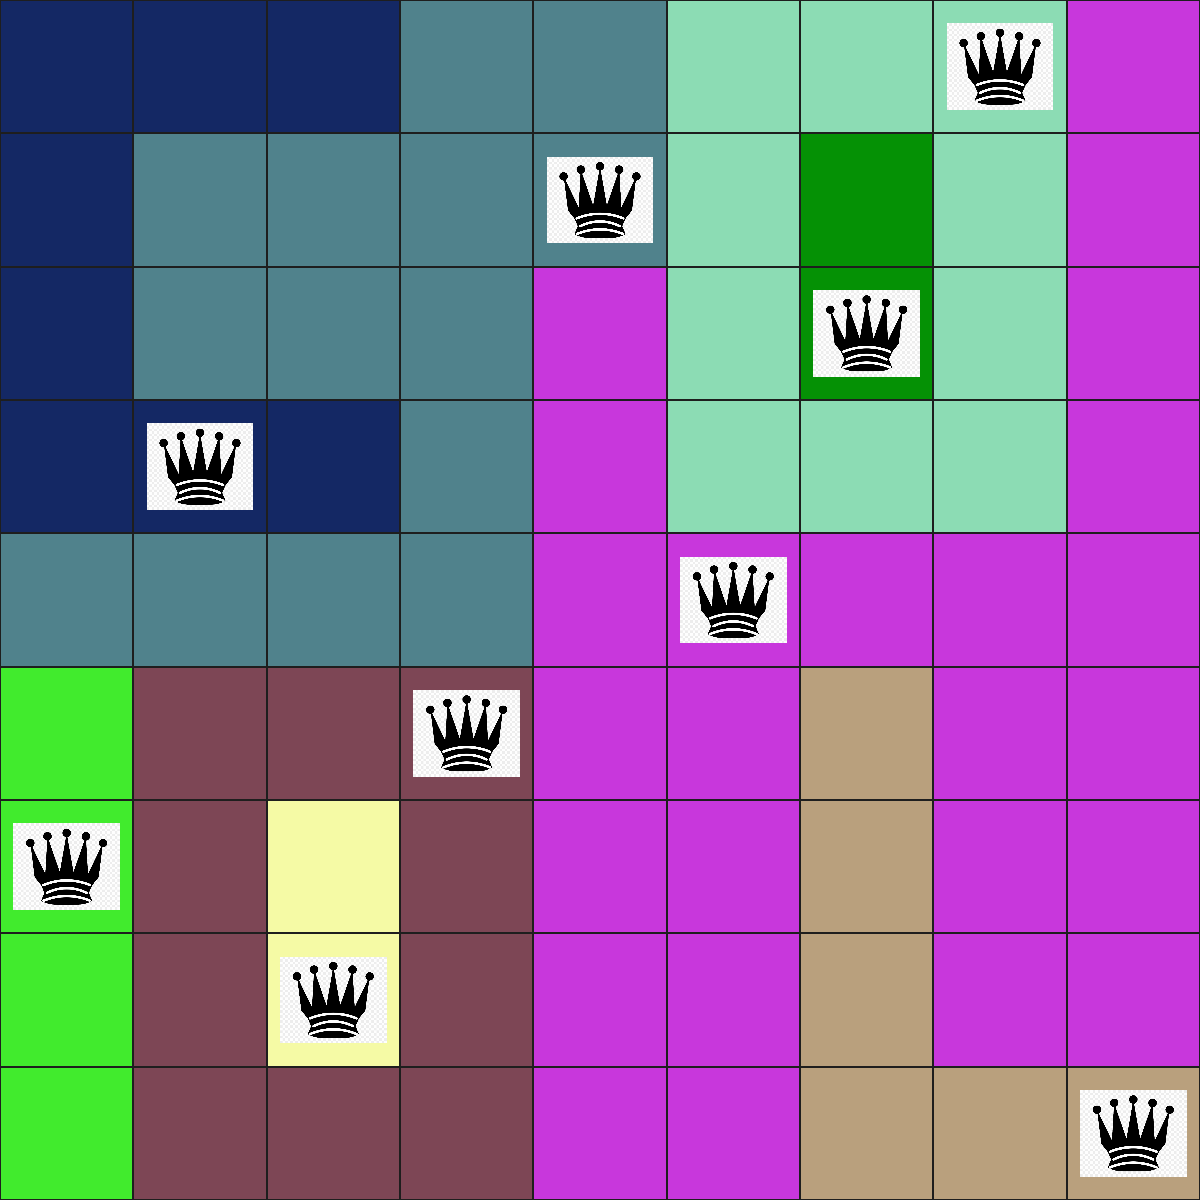
\includegraphics[width=10cm]{figures/out1.png}
    \caption{Output GUI --- Test 1}
\end{figure}

\section{Test 2: Papan berukuran $11\times 11$ (in2.txt)}

Test case ini menggunakan papan berukuran $11\times 11$ dimana setiap baris merupakan satu region warna. 

\begin{table}[H]
    \centering
    \captionof{table}{Input Test 2}
    \renewcommand{\arraystretch}{1.2}
    \setlength{\tabcolsep}{20pt}
    \begin{tabular}{|l|}
        \hline
        \phantom{text}\\
        AAAAAAAAAAA\\
        BBBBBBBBBBB\\
        CCCCCCCCCCC\\
        DDDDDDDDDDD\\
        EEEEEEEEEEE\\
        FFFFFFFFFFF\\
        GGGGGGGGGGG\\
        HHHHHHHHHHH\\
        IIIIIIIIIII\\
        JJJJJJJJJJJ\\
        KKKKKKKKKKK\\
        \phantom{text}\\
        \hline
    \end{tabular}
\end{table}

Setiap baris terdiri dari satu huruf yang sama (11 kolom), sehingga setiap baris adalah satu region warna.

Program menyediakan dua format output: file teks (.txt) dan gambar (.png).

\subsection*{Output sebagai File TXT}
\begin{lstlisting}[basicstyle=\ttfamily\small]
#AAAAAAAAAA
BB#BBBBBBBB
CCCC#CCCCCC
D#DDDDDDDDD
EEE#EEEEEEE
FFFFF#FFFFF
GGGGGGG#GGG
HHHHHHHHH#H
IIIIII#IIII
JJJJJJJJ#JJ
KKKKKKKKKK#

Waktu pencarian: 17135 ms
Banyak kasus yang ditinjau: 5599053306 kasus
\end{lstlisting}

\subsection*{Output sebagai Gambar (PNG)}
\begin{figure}[H]
    \centering
    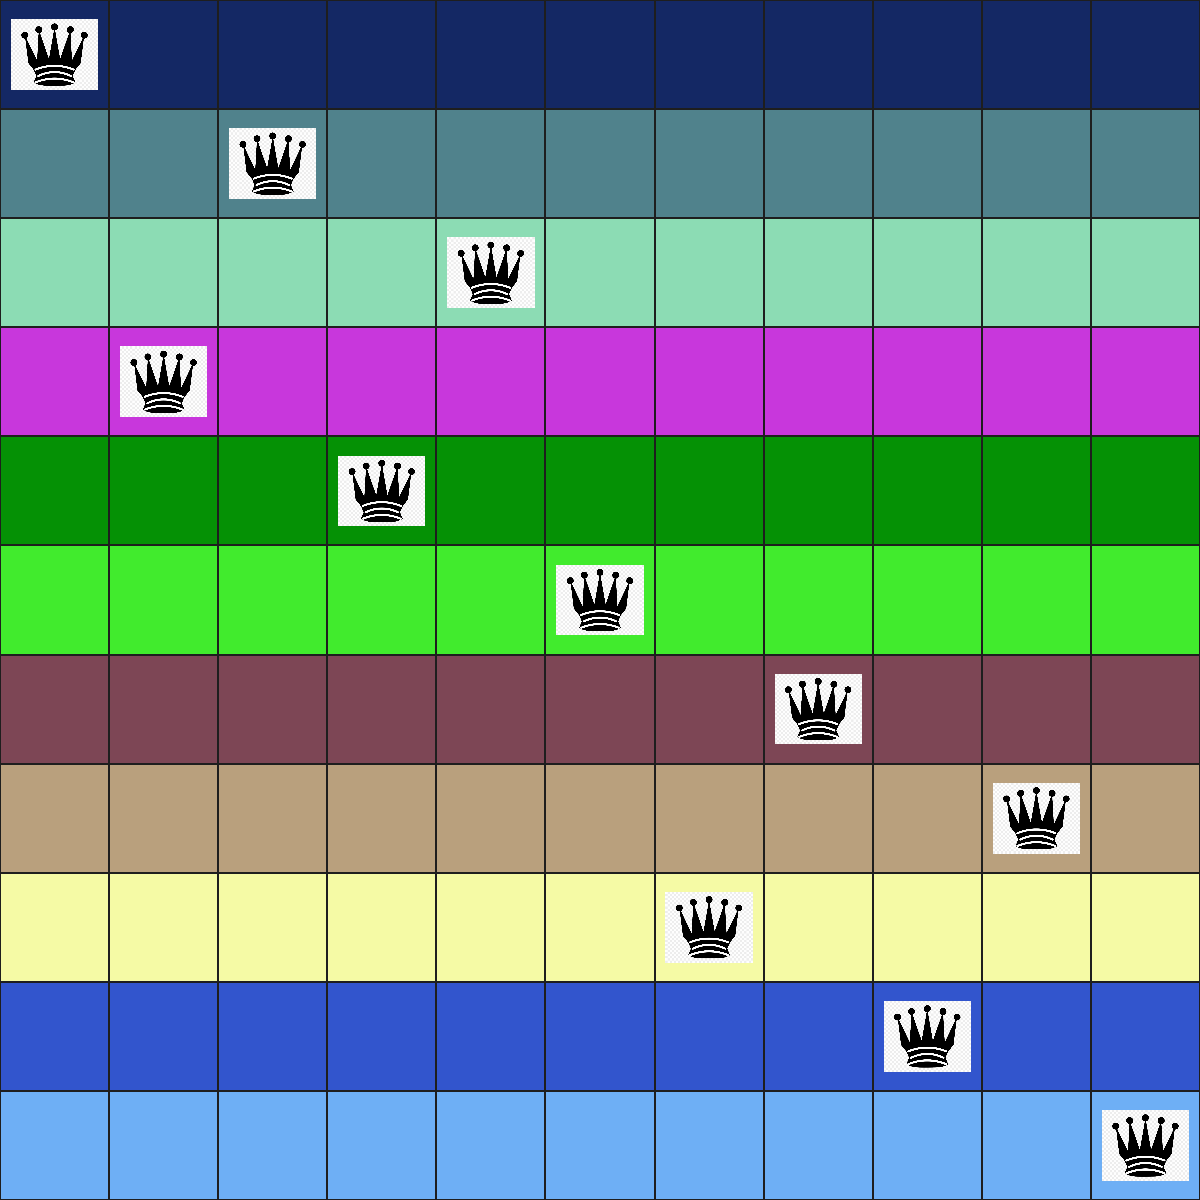
\includegraphics[width=10cm]{figures/out2.png}
    \caption{Output GUI --- Test 2}
\end{figure}

\section{Test 3: Papan berukuran $1\times 1$ (in3.txt)}

\begin{table}[H]
    \centering
    \begin{minipage}{0.45\textwidth}
        \centering
        \captionof{table}{Input Test 3}
        \renewcommand{\arraystretch}{1.2}
        \setlength{\tabcolsep}{40pt}
        \begin{tabular}{|l|}
            \hline
            \phantom{text}\\
            A\\
            \phantom{text}\\
            \hline
        \end{tabular}
    \end{minipage}
\end{table}

Papan berukuran $1\times 1$ dengan satu region. Queen langsung ditempatkan pada satu-satunya sel.

Program menyediakan dua format output: file teks (.txt) dan gambar (.png).

\subsection*{Output sebagai File TXT}
\begin{lstlisting}[basicstyle=\ttfamily\small]
#

Waktu pencarian: 0 ms
Banyak kasus yang ditinjau: 1 kasus
\end{lstlisting}

\subsection*{Output sebagai Gambar (PNG)}
\begin{figure}[H]
    \centering
    
\includegraphics[width=10cm]{figures/out3.png}
    \caption{Output GUI --- Test 3}
\end{figure}

\section{Test 4: Papan berukuran $9\times 9$ --- Tidak Ada Solusi (in4.txt)}

\begin{table}[H]
    \centering
    \begin{minipage}{0.45\textwidth}
        \centering
        \captionof{table}{Input Test 4}
        \renewcommand{\arraystretch}{1.2}
        \setlength{\tabcolsep}{40pt}
        \begin{tabular}{|l|}
            \hline
            \phantom{text}\\
            ABCDEFGHI\\
            BBCDEFGHI\\
            CCCDDEFGH\\
            DDDDDDEGH\\
            EEEEEFGHH\\
            FFFFFFGHH\\
            GGGGGGGHH\\
            HHHHHHHII\\
            IIIIIIIII\\
            \phantom{text}\\
            \hline
        \end{tabular}
    \end{minipage}
\end{table}

Karena papan ini tidak memiliki solusi yang valid (region tidak memungkinkan penempatan queen yang memenuhi semua aturan), program tidak menghasilkan file solusi .txt.

\subsection*{Output sebagai Gambar (PNG)}
\begin{figure}[H]
    \centering
    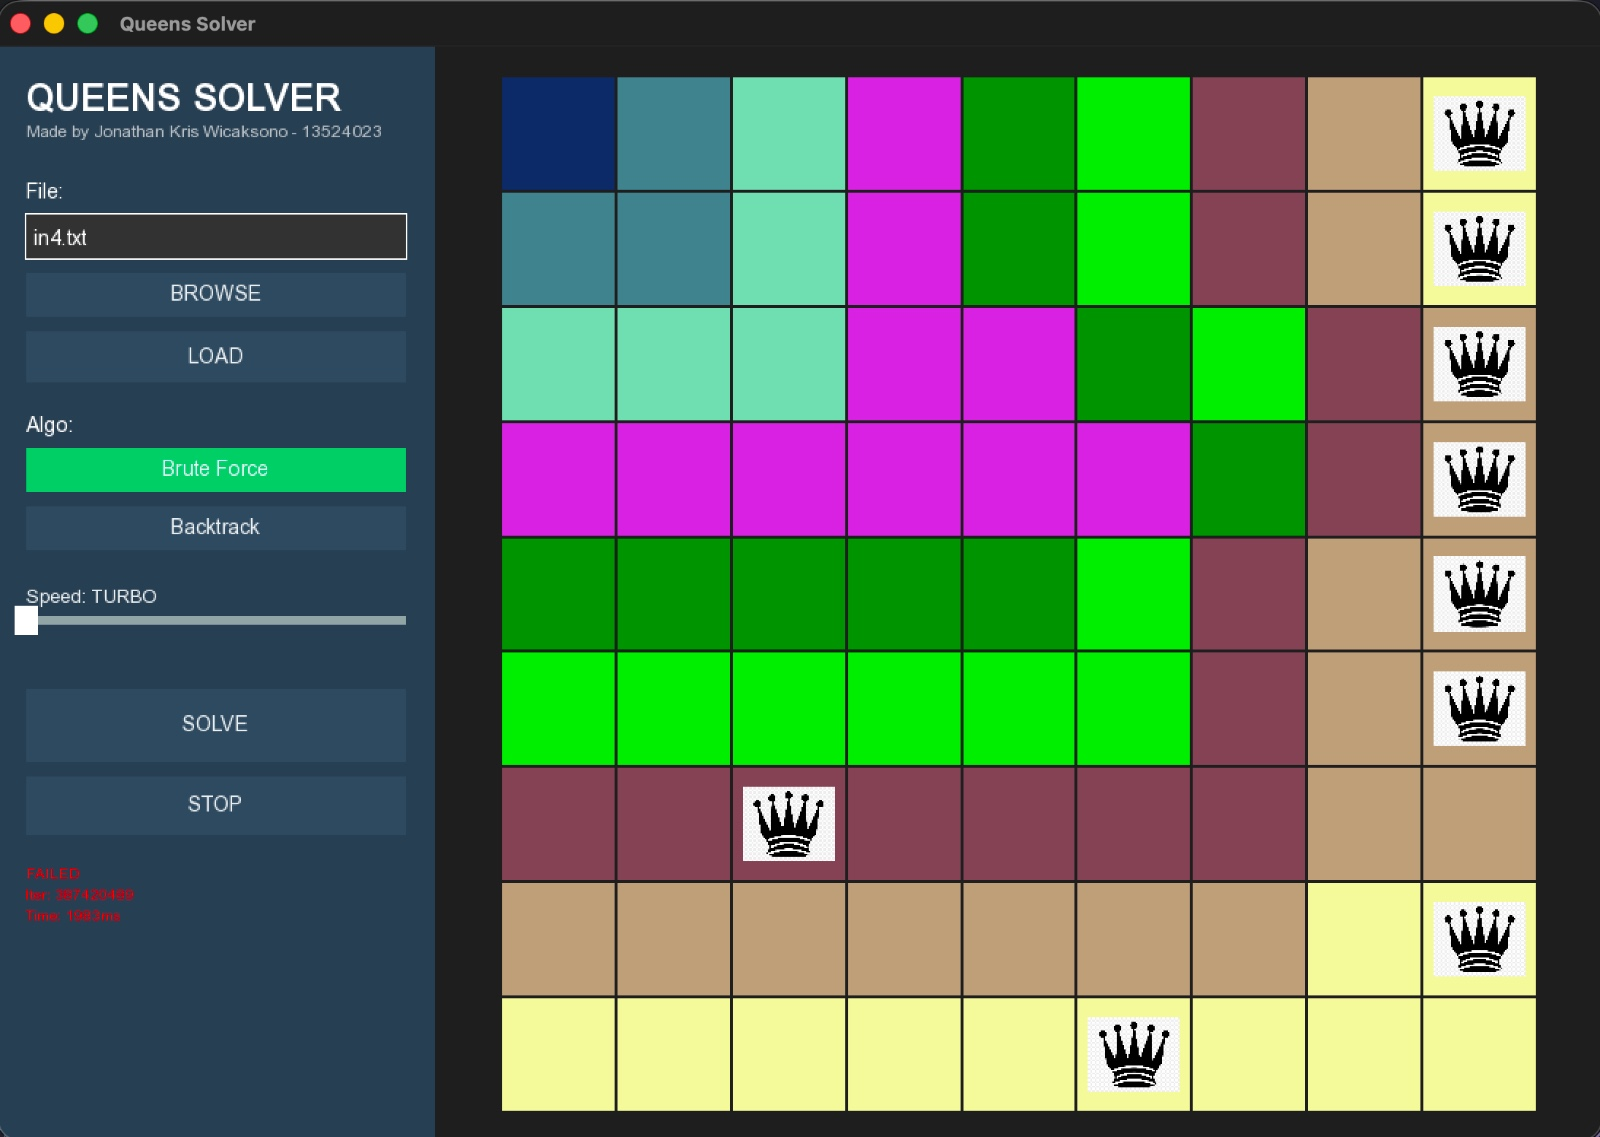
\includegraphics[width=10cm]{figures/out4.png}
    \caption{Output GUI --- Test 4 (Tidak Ada Solusi)}
\end{figure}

\section{Test 5: Input Tidak Valid --- Panjang Baris Berbeda (in5.txt)}

\begin{table}[H]
    \centering
    \begin{minipage}{0.45\textwidth}
        \centering
        \captionof{table}{Input Test 5}
        \renewcommand{\arraystretch}{1.2}
        \setlength{\tabcolsep}{30pt}
        \begin{tabular}{|l|}
            \hline
            \phantom{text}\\
            ABCDEFGHIJJ\\
            BBCDEFGHI\\
            CCCDDEFGH\\
            DDDDDDEGH\\
            EEEEEFGHH\\
            FFFFFFGHH\\
            GGGGGGGHH\\
            HHHHHHHII\\
            IIIIIIIII\\
            \phantom{text}\\
            \hline
        \end{tabular}
    \end{minipage}
\end{table}

Program berhasil mendeteksi bahwa input tidak valid karena panjang baris tidak konsisten, dan menampilkan pesan error pada panel status GUI.

Karena input tidak valid, program tidak menghasilkan file solusi .txt. Output hanya berupa pesan error yang ditampilkan di GUI.

\subsection*{Output sebagai Gambar (PNG)}
\begin{figure}[H]
    \centering
    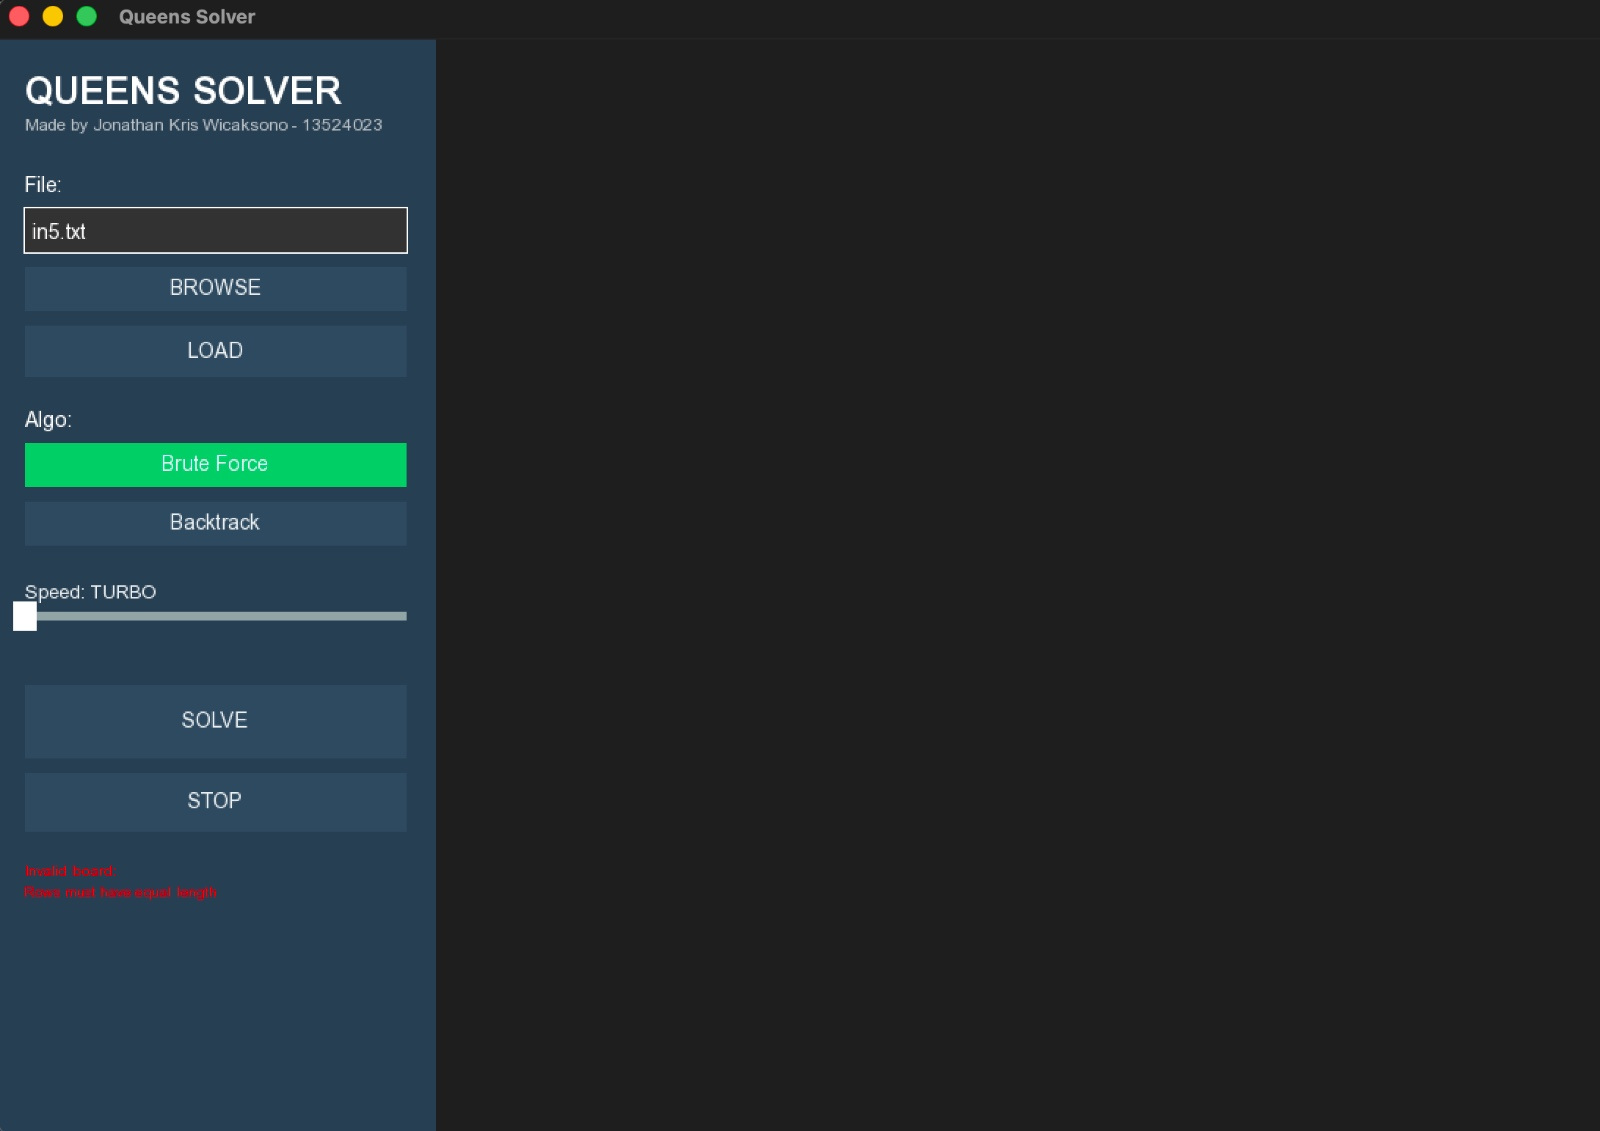
\includegraphics[width=10cm]{figures/out5.png}
    \caption{Output GUI --- Test 5 (Input Tidak Valid)}
\end{figure}
